% status: 90%
% chapter: TBD

\title{Power BI}

\author{Surya Prakash Sekar}
\affiliation{%
  \institution{Indiana University
  Bloomington} \city{Bloomington} \state{Indiana} \postcode{47408} \country{USA}
  }
\email{sursekar@iu.edu}

% The default list of authors is too long for headers}
\renewcommand{\shortauthors}{Surya Prakash Sekar}

\begin{abstract}
Power BI is a business analytics tool offered by Microsoft. It is mainly used 
in the industry for analysing data, creating interactive dashboards for 
visualization, business intelligence features and its wide range of cloud 
services. It is notable for its ability to connect with a wide range of data 
sources on the cloud, data preparation capabilities and extracting business 
insights from the data.
\end{abstract}

\keywords{hid-sp18-418, visualization, data model, cloud services}
%use up to 5 keywords

\maketitle

\section{History}
Power BI was launched by Microsoft in September 2013 as Power BI for 
Office 365. The initial release of Power BI was based on the Microsoft 
Excel–based add-ins: Power Query, Power Pivot and Power View. Microsoft kept 
adding many additional features like Question and Answers, enterprise level 
data connectivity and security options via Power BI Gateways throughout time. 
Power BI was first released to the public on July 2015 
~\cite{hid-sp18-418-power bi-history}.

\section{Introduction}
Power BI facilitates the creation of interactive visualizations, reports and 
dashboards that are shared across the cloud, also features to type 
natural-language questions about the data on the dashboard, handling files 
that are too large for Excel are available in it ~\cite{hid-sp18-418-power bi
-intro}.
Power BI includes both a desktop program and a cloud service. The cloud service 
is multi-platform which runs on Microsoft Edge, Internet Explorer, Chrome, 
Safari for Mac and Firefox. There are also mobile apps for iOS, Android and 
Windows that enables viewing of the Power BI or SQL Server Reporting Services 
reports and dashboards.
\section{Terminologies}
Power Query - Power Query is an Excel add-in that can be used for data 
discovery, data reshaping and aggregating the data from various sources. 
Power Query is one of the Excel add-ins provided as part of Microsoft Power 
BI self-service solution ~\cite{hid-sp18-418-power bi-intro}.
DAX –  Data Analysis Expression, is a formula language. DAX is used to define 
custom calculations for calculated columns and measures. DAX includes some of 
the formulas used in excel ~\cite{hid-sp18-418-dax-basics}.
Content Pack -  It is a collection of pre-defined visualizations and reports 
with respect to certain sample data sources.
Quick Insights – It is a functionality within Power BI which enables it to 
deep dive into the dataset for hidden insights and display the 
visuals accordingly.
PowerPivot - PowerPivot uses an in-memory engine called VertiPaq. 
This SSAS engine takes advantage of the increased RAM available in the 
PC thus enabling the calculations and the aggregations to be comparatively 
faster, it works on DAX ~\cite{hid-sp18-418-power pivot}.
Power View – Power View is a data visualization technology that allows the 
creation of interactive charts, graphs, maps, and other visuals which is 
very effective in Ad-hoc analysis.
R-Powered Visuals – R code can be written to construct visualizations 
using Power BI.

\section{Components}

\subsection{Power BI Desktop}
Power BI Desktop is used to create reports and data visualizations on
the dataset, it is a desktop-based application.

\subsection{Power BI Gateway}
Power BI on-premises gateway is used to keep the data fresh 
by connecting to on-premise data sources without needing to move the data. It 
enables querying large datasets and benefiting from the existing investments
~\cite{hid-sp18-418-power bi-components}.

\subsection{Power BI Mobile Apps}
Power BI mobile apps can be used to view the dashboards 
and the data in mobile phones. Power BI apps are available across Windows, iOS,
and Android platform. The dashboards are automatically rescaled with respect 
to our devices.

\subsection{Power BI Service}
Power BI Service is a cloud service and is mainly used to publish the 
Power BI reports and data visualizations on the cloud 
~\cite{hid-sp18-418-power bi-components}.

\subsection{Power BI Embedded}
Power BI REST API can be used to build dashboards and 
reports into the custom applications that serves Power BI users
~\cite{hid-sp18-418-power bi-components}. It could also be used for non-Power 
BI users as well.

\section{Installation}
We need a work or university email id to download Power BI Desktop. It can be 
downloaded at https://powerbi.microsoft.com/en-us/get-started/ .The basic 
version of Power BI with cloud service is available for free which offers 
1GB data storage which can be expanded through a paid account. Also, it extends
its automated data refresh, increased streaming capacity features to the paid 
accounts. The published dashboards will be available on the cloud and can be 
accessed from https://app.powerbi.com
 
\section{Key Features}
Power BI desktop additionally offers basic data wrangling capabilities like 
Excel's Power Query. It can work with some unique data types like Salesforce, 
Google Analytics, MailChimp, GitHub, QuickBooks online and pull them from the 
cloud. ~\cite{hid-sp18-418-power bi-intro}.
It has the capability to run R script files as well, indicating that any data 
that could be extracted by R can be imported into Power BI as well. 
Organizations can create their own content packs for getting data from their 
on-premise systems and the cloud services they use. What the content packs do 
is give Power BI the data model of the services it gets data from, so it can 
automatically build dashboards and charts to expose useful data, and so you 
can use the natural language Q&A feature. Power Q&A is a natural language 
engine for the data model that we create in Power BI. Users can ask questions 
and answers would be processed and output with respect to the data model.Once 
the data model has been deployed into the Power BI website, then users can ask 
questions and get answers on the model ~\cite{hid-sp18-418-power bi-intro}.
The author of the dashboard can grant different types of access with respect 
to the hierarchy of the viewer based on the row level security concept within 
Power BI, which restricts data access depending upon the user.

 
\section{Dashboard Sample}
A toy dashboard using quick insights on Power BI using the sample Human 
Resource data available on it has been created, the dashboard and the report 
analyses the new hires, active employees and employees who quit to discover 
trends and insights with respect to the hiring strategy. The dashboard has 
been published online and can be viewed using a Power BI account at 
https://app.powerbi.com/groups/me/dashboards/9fd80216-7d17-4bb9-a6d3-f47ddb6
61971

\begin{figure}[!ht]
  \centering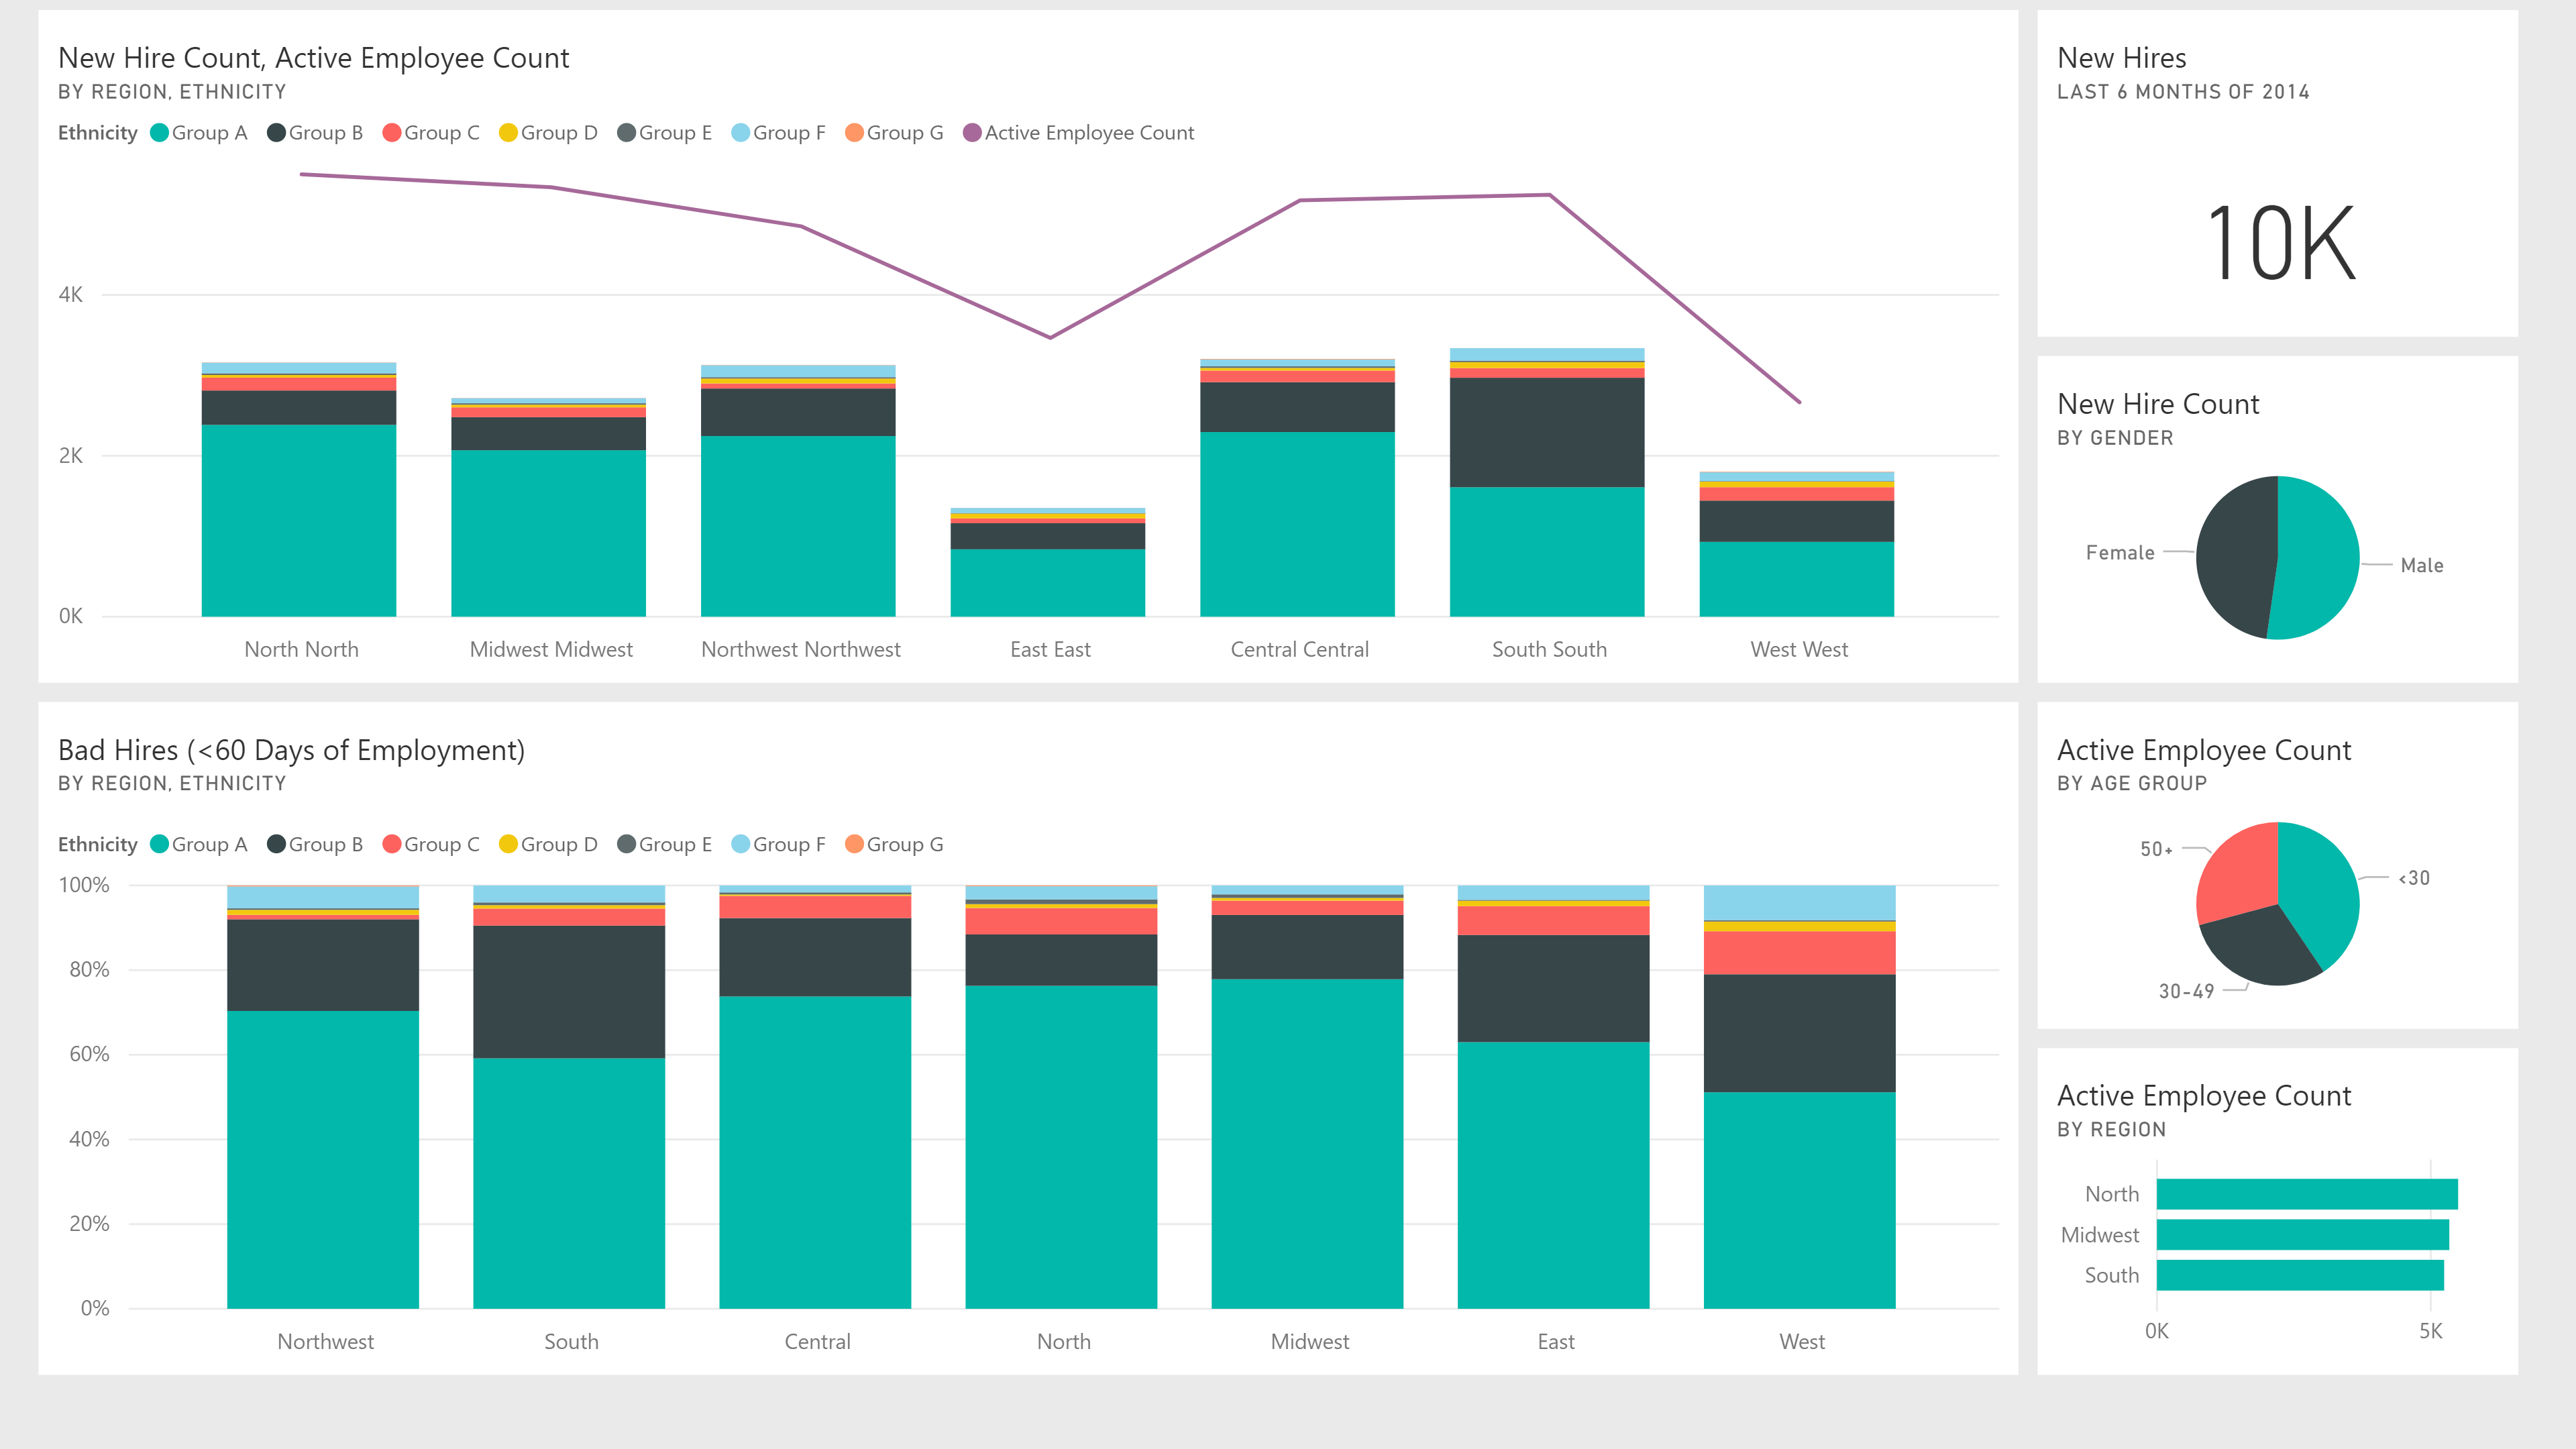
\includegraphics[width=\columnwidth]{image/dashboard.png}
  \caption{Sample Dashboard}\label{f:Dashboard}
\end{figure}

The reports for the dashboard have also been published and the link to the 
reports for the sample Power BI dashboard is available below, this report 
can be viewed by anyone
https://app.powerbi.com/view?r=eyJrIjoiMWNlNWRkOTQtOWFhNS00NWU4LWEwMzctYWQ
zMTczNTk1ODhiIiwidCI6IjExMTNiZTM0LWFlZDEtNGQwMC1hYjRiLWNkZDAyNTEwYmU5MSIsI
mMiOjN9

 
\section{Conclusion}
Power BI in overall is being used as a cloud-based analytics environment which 
can be employed to solve a wide range of problems related to business analysis 
and automated cutting-edge data visualizations. The extravagant features 
available offers Power BI an edge over its fellow competitors like Tableau, 
Qlikview and so on. The options to automate most of the operations makes 
Power BI the go to platform when it comes to building data models and sharing 
dashboards on the cloud in the industry.
 

\begin{acks}

The authors would like to thank Dr.~Gregor~von~Laszewski for his
support and suggestions to write this paper.

\end{acks}

\bibliographystyle{ACM-Reference-Format}
\bibliography{report} 
